\chapter{Detección óptica de caracteres (OCR)}
En este capitulo se pretende explicar que es el OCR, obtener una idea basica
de los distintos algorimos que se pueden implementar para
utilizar esta tecnica, para luego centrarnos en la red convolucional entrenada por
Ankandrew [referencia al git], con la idea de finalizar en un algoritmo en Python 3
que permita obtener los caracteres de una patente mediante una imagen.

\section{Algoritmos de OCR}
Como primera instancia vamos a definir que es OCR, por sus siglas en ingles Optical character
Recognition o en español Reconocimiento Optico de caracteres, es una tecnica que permite
obtener texto en un formato editable para una maquina(ASCII o Unicode)a partir de una imagen
de texto.
Para logarlo el software inspecciona la imagen buscando formas que coincidan con la forma
de los caracteres, y dependiendo del tipo de software las compara con una base disponible
para el programa o trata de identificarlos mediante el analisis de sus caracteristicas.
La tecnologia más utiliza para realizar el OCR es la de Redes Neuronales, ya sea
mediante redes LSTM por sus siglas en ingles Long-Short Term Memory, que son una variedad de Redes
neuronales recurrentes o bien CNN por sus siglas en ingles Convolutional Neural Network, o en español Red
Neuronal Convolucional.

Si bien el fin ultimo de ambos tipos de red es obtener los caracteres a partir de la imagen,la forma en
trabajan difiere significamente, las redes LSTM almacenan informacion de estados anteriores mediante bucles,
lo que les permite realizar predicciones de estados futuros usando informacion pasada almacenada y la informacion
del estado actual.
\begin{figure}[h]
    \centering
    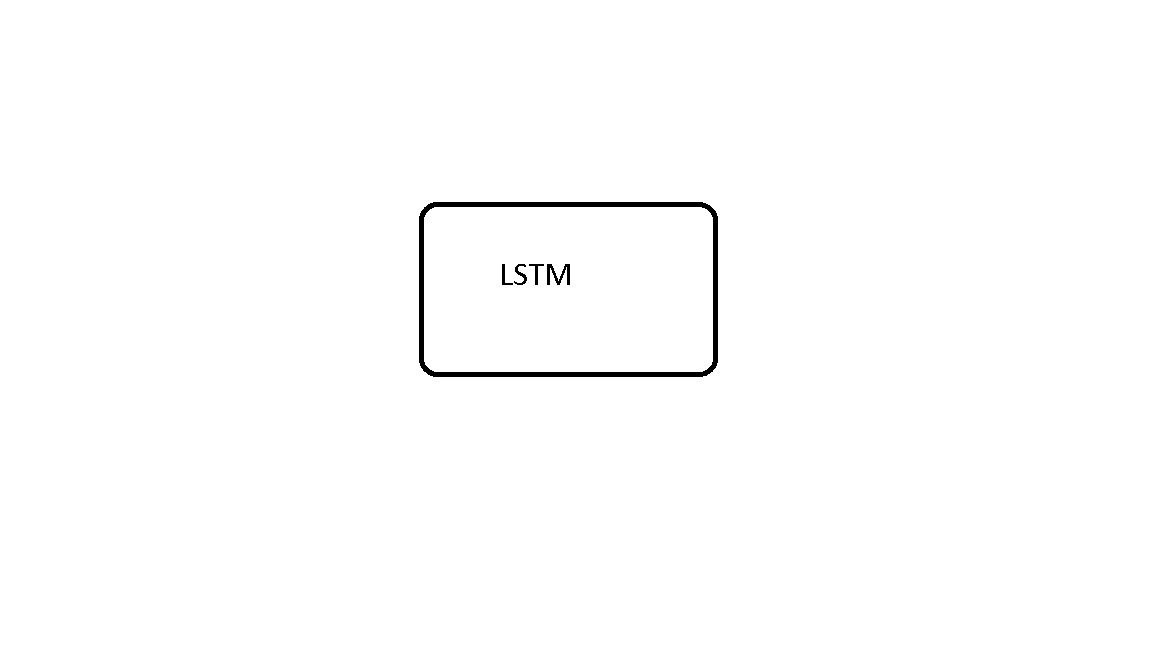
\includegraphics[width=0.25\textwidth]{imgs/LSTM-diagrama.jpg}
    \label{fig:diagrama-LSTM}
    \caption{Diagrama basico red LSTM.}
\end{figure}
Este tipo de redes son las mas utilizadas actualmente para realizar reconocimiento de
caracteres, pero cuentan con la desventaja de requerir mayor poder de computo, por la necesidad
almacenar y anidar datos anteriores.

La otra alternativa que se utiliza es la de Redes Neuronales del tipo convulucional, que mediante
el uso de convoluciones entre los pixeles de la imagen y una serie de matrices establecidas
extrae caracteristicas utilizadas para comparar la imagen con una lista de valores posibles,
dando por resultado el caracter que mas similitud tenga con el set de comparacion.
\begin{figure}[h]
    \centering
    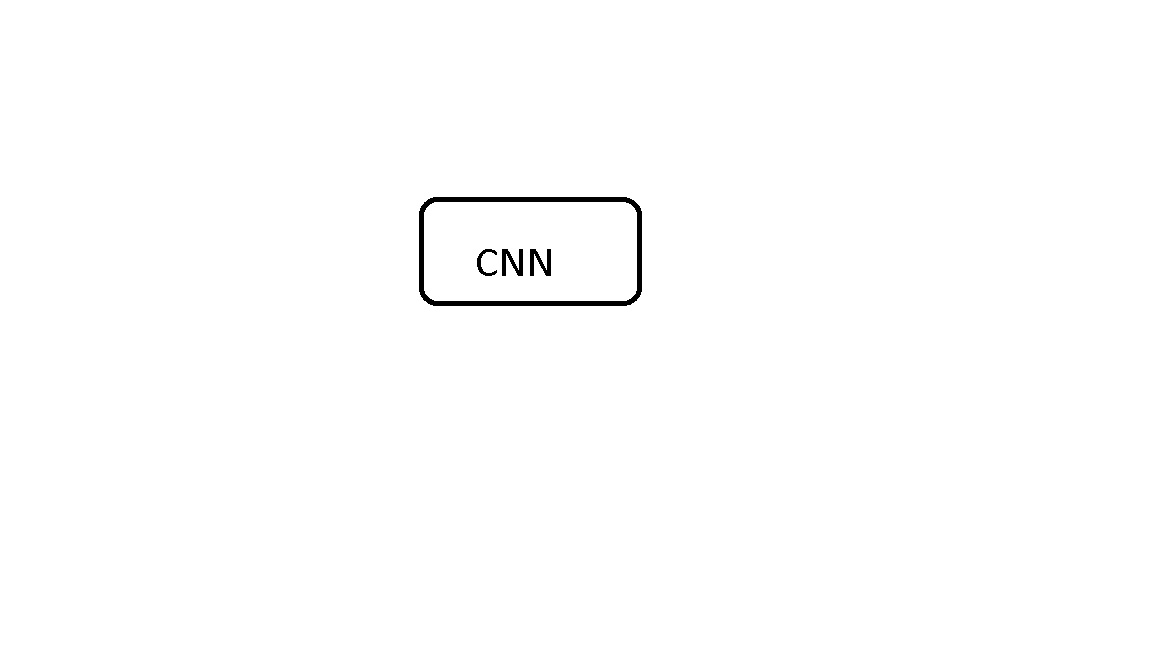
\includegraphics[width=0.25\textwidth]{imgs/CNN-diagrama.jpg}
    \label{fig:diagrama-CNN}
    \caption{Diagrama basico red CNN.}
\end{figure}

Al no requerir almacenar informacion ni trabajar de forma recursiva, la implementacion
de este tipo de redes pueden ser implementadas en equipos con un hardware de menor potencia,menor tamaño y
por consiguiente menor costo.

Por lo que esta ultima opcion es de las mas utilizadas a la hora de colocar en sistemas embedidos de baja
potencia, o que por cuestiones de energia tengan un consumo menos reducido. Como el objetivo de nuestro PIP el diseño
de un sistema que pueda ser utilizado en diferentes entornos, se considero que esta era la mejor opcion para
el desarrollo.

De varios algoritmos encontrados que realizan OCR mediante redes neuronales convolucionales, se encontro uno
preentrenado para la deteccion de patentes argentinas, tanto para la versiones antiguas del año 1994 como para la version moderna del
mercosur del año 2015, las cuales se pueden ver en la Fig. \ref{fig:patentes-arg}. [https://www.iprofesional.com/autos/376250-como-saber-el-ano-de-un-auto-por-la-patente-en-argentina]
\begin{figure}[h]
    \centering
    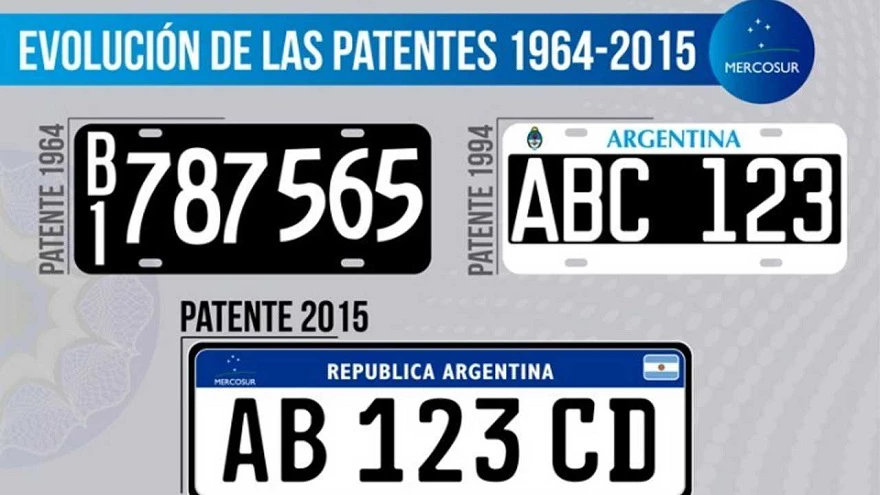
\includegraphics[width=0.5\textwidth]{imgs/patentes-arg.png}
    \caption{evolucion Patentes Argentinas.}
    \label{fig:patentes-arg}
\end{figure}

Este algoritmo como se menciono al inicio del capitulo fue entrenado por Ankandrew, el cual es un modelo convencional de red convolucional
formada por un bloque convolucional, luego un bloque Batch-Normalization, una funcion de activacion, seguida por un bloque de MaxPooling
continuada por un bloque GlobalAvgPooling para finalizar en una bloque softmax conectado mediante una Fully Connect Layer de 37x7, esto surge de que maximo se poseen 7 caracteres
de salida y el 37 de la suma de las 26 letras del abcedario, los 10 numeros del 0 al 9 y el simbolo $\_$ utilizado para el caso de las patentes antiguas
que solo poseen 6 caracteres, todos los terminos descriptos anteriormente seran explicados en la siguiente seccíon.

\section{Marco teórico}
Como se viene mencionando durante las secciones anteriores se usara una red neuronal del tipo convolucional para realizar el algoritmo de OCR,
pero bien para comprender como trabaja un red convolucional es necesario saber primero que es una red neuronal y como esta se constituye.

Entonces ¿qué es una red nueronal?, se define entonces como red neuronal a un algoritmo computacional recursivo que intenta imitar el cerebro
humano, en otras palabras es un algoritmo de computación compuesto por un gran numero de elementos simples que se
encuentran interconectados, los cuales procesan la información por medio de estados dinámicos, respondiendo a entradas externas, que permite
clasificar datos en un numero finito de clases o categorias.esquematizado en
la Fig. \ref{fig:esquema-redes}.
\begin{figure}[h]
    \centering
    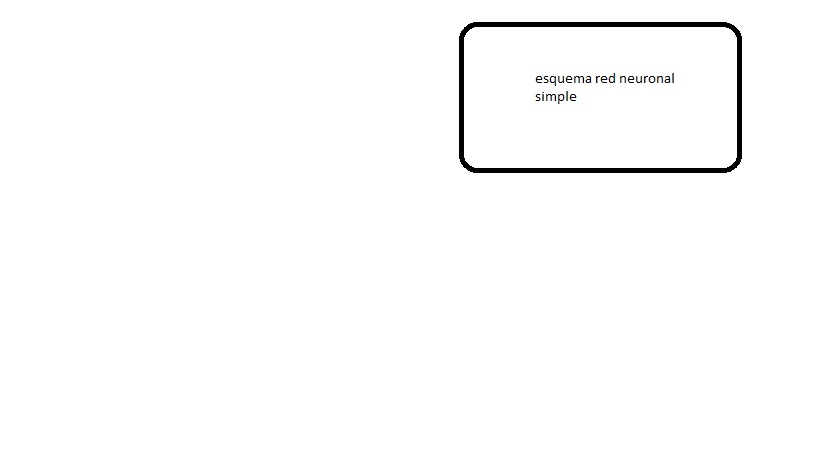
\includegraphics[width=0.5\textwidth]{imgs/Redes-esquema.jpg}
    \caption{Esquema simplificado de una red neuronal.}
    \label{fig:esquema-redes}
\end{figure}
Debido a la semenjanza que existe entre los algoritmos de Deep Learning (algoritmos de aprendizaje computacional o
Machine learning [Referencia https://www.ibm.com/topics/machine-learning] compuesto por redes neuronales
de 3 o mas capas)[Referencia https://www.ibm.com/es-es/topics/deep-learning] y el cerebro humano , a la
unidad fundamental de estos sistemas se la denomina neurona, apreciado en la Fig. \ref{fig:comparativa-neuronas}
\begin{figure}[h]
    \centering
    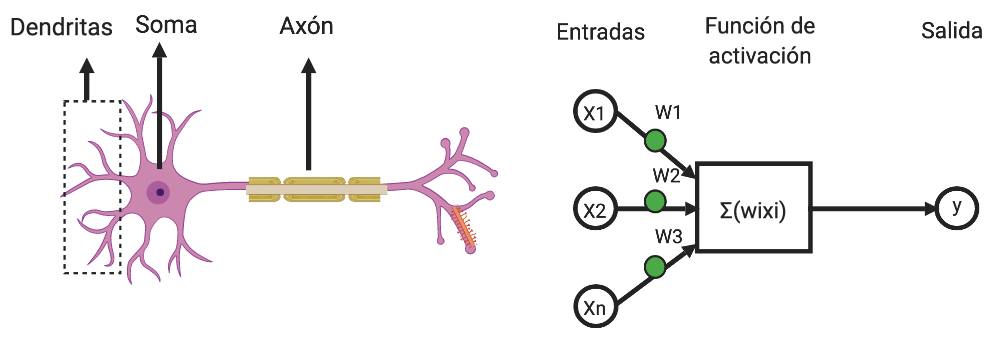
\includegraphics[width=1\textwidth]{imgs/comparacion-neurona-red.png}
    \caption{Comparacion neurona biologica con nuerona artificial.}
    \label{fig:comparativa-neuronas}
    %https://futurelab.mx/redes%20neuronales/inteligencia%20artificial/2019/06/25/intro-a-redes-neuronales-pt-1/
\end{figure}
Cada neurona o unidad fundamental de la red procesa la información de un grupo de neuronas previas y la entrega al siguiente grupo,este proceso
se puede entender como la sinapsis neuronal de los seres vivos.

La sinapsis entre nueronas es una suma poderada que puede ser expresada como $Y =W^T\dot X + b$ donde $Y$ es el vector de salida de la nuerona,
$W$ representa los pesos de la neurona, $b$ es un bias y $X$ es el vector de entrada.
Es posible realizar un arreglo en paralelo de neuronas, lo cual recibe el nombre de capa,las capas se interconectan para crear redes
más complejas capaces de realizar tareas más especificas Fig.\ref*{fig:esquema-redes}.

Debido a que en esencia el proceso que realiza la neurona es una transformación lineal, al interconectar capas la resultante sigue siendo
una transformación lineal. Este problema de linealidad se soluciona aplicando una función de activación o transformacion no lineal,
luego de la transformación lineal, obteniendo $Y= f(W^T \dot X + b)$, algunas de estas funciones las podemos ver en la
Fig. \ref*{fig:funciones-activacion}.
\begin{figure}
    \centering
    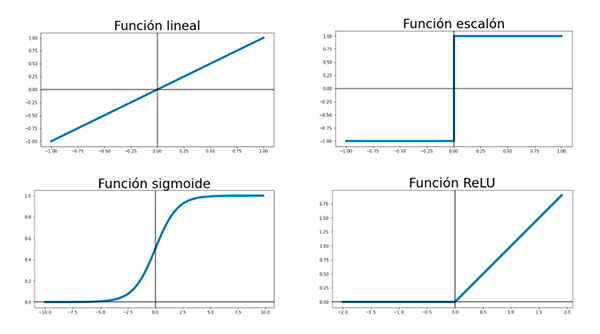
\includegraphics[width=1\textwidth]{imgs/Funciones-de-activacion.jpg}
    \caption{Funciones de activacion más comunes.}
    \label{fig:funciones-activacion}
\end{figure}
En forma resumida podemos decir que la red funciona de la siguiente manera, se realiza la multiplacion de la entrada y los pesos de la red,
luego los resultados son ingresados a la funcion de activacion para quitar las linealidades, a su vez se calcula una funcion de costo que se obtiene
con los valores obtenidos y los que se espera obtener, esta funcion es usada principalmente en el ajuste de los pesos de la red, es decir el
entrenamiento de la misma.
Como este trabajo esta centrando en el trabajo con imagenes las redes mas utilizadas son las redes neuronales de convolución o
CNN Convolutional Neuronal Network por sus siglas en inglés, ya que su diseño se basa en la estructura de la corteza visual animal, esta
imitación se consigue utilizando convoluciones bidimensionales. Este tipo de redes poseen caracteristicas que las hacen unicas, por lo que
se prodece a continuacion a enumerar las partes que la componen y se muestra un esquema de la misma en la Fig. \ref*{fig:esquema-CNN}
\begin{itemize}
    \item Capa convolucional: capa principal de las CNN, sus parametros son basicamente filtros entrenables de dimesiones determindas por el
          usuario,realizando una multiplicacion punto a punto recorriendo toda la dimesion, produciendo un mapa de activacion bidimensional, en la
          Fig. \ref{fig:esquema-capa-convolucional} se ve el funcionamiento de esta capa. Cada uno de estos filtros se activara segun la
          caracteristica que se busque.
    \item Capa de agrupacion: se coloca entre las capas de convolucion, toma los mapas de caracteristicas producidos por la capa de
          convolucion y los agrupa en una imagen. En esta capa se produce una reduccion de la dimesion, lo que reduce la complejidad 
          para evitar el sobreajuste de los parametros.
    \item Capa de activacion: la unica funcion de esta capa es la de aumentar la no linealidad sin modificar los parametros, no son entrenables
          por lo que por ella solo se propagan los errores calculados.
    \item capa completamente conectada: tiene la estructura comun de una capa de nueronas pero con las particularidad que todas las neuronas
          de esta capa estan conectadas a todas las neuronas de la capa anterior.
\end{itemize}
\begin{figure}
    \centering
    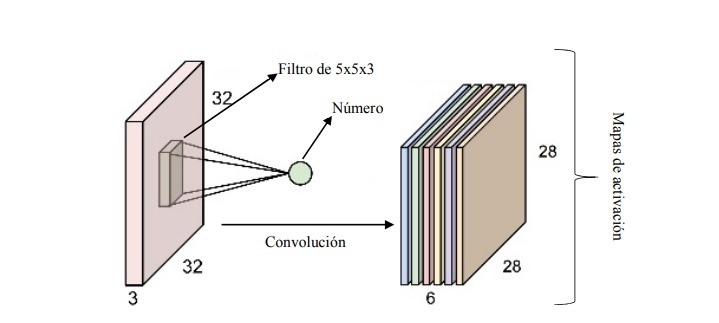
\includegraphics[width=1\textwidth]{imgs/capa-convolucional.jpeg}
    \caption{Esquema de funcionamiento de una capa convolucional.}
    \label{fig:esquema-capa-convolucional}
\end{figure}
\begin{figure}
    \centering
    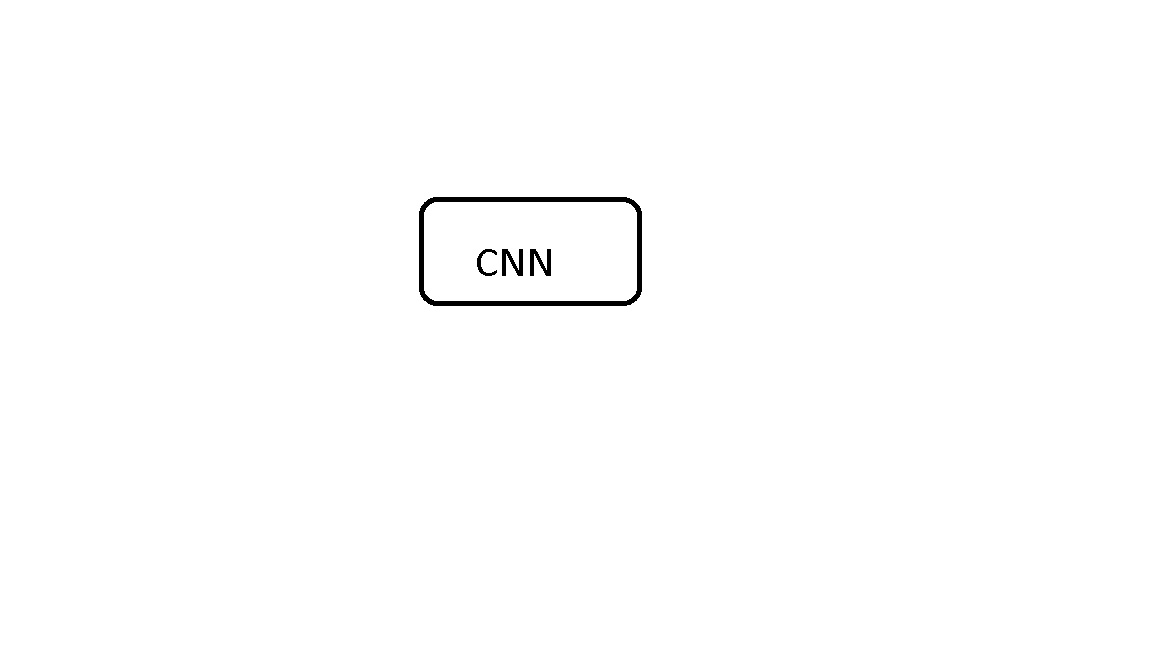
\includegraphics[width=1\textwidth]{imgs/CNN-completa.jpg}
    \caption{Esquema de un red del tipo CNN.}
    \label{fig:esquema-CNN}
\end{figure}
Antes de continuar haremos una pausa para explicar el comportamiento de la convolución bidimensional, es similar al caso conocido en 1D pero
en este caso se desplaza una submatriz de un tamaño predefinido, comunmente denonimado kernel.

Se define filtro, o kernel a la respuesta de un sistema discreto, el filtro es de dimensión $2k x 2k$ donde $k$ es un
valor establecido arbitrario (usualmente son matrices cuadradas de $3x3$ o $5x5$) que define cuantos valores habra de la muestra.

Se define a $h[n]$ como un filtro de dimension $2k x 2k$ e $I$ una imagen a escala de grises, donde cada punto de coordenadas $(i,j)$ es el
resultado de la convolucion entre $h$ e $I$ dado por
\begin{equation}
    O(i,j)= \sum_{u=-k}^{k} \sum_{v=-k}^{k} h(u,v)I(i-u,j-v)
\end{equation}

Esta operacion consiste en filtrar una imagen de dimension $(2k+1)x(2k+1)$ en la imagen $I$ para cada pixel centrado en dicha imagen,
calculando la operacion de convolucion.
El ajustes de los filtros necesarios para extraer caracteristicas puede resultar un proceso largo y tedioso que no siempre conduce a los
resultados que uno esperaria, por lo que se puede utilizar machine learning para obtener los valores optimos de los filtros.
Este bloque de filtros es el que se denomino bloque de convolucion que fue nombrado en la seccion anterior.
Otro de los bloques que necesitamos mencionar es el de Batch-Normalization[https://keepcoding.io/blog/batch-normalization-red-convolucional/], 
este puede ser definido como una tecnica que busca reducir el cambio de covariables internas o internal covariate shift, esto con la finalidad 
de hacer mas robusta la red a una mala eleccion de valores iniciales. El internal covariate shift se define como el cambio en la distribucion de la activacion de la red, 
esto se logra en la etapa del entrenamiento,ingresando pequeños grupos de datos de entrada o mini-batches.

En términos matemáticos, lo que se hace es centrar y normalizar cada mini-batch ingresa a la red con una media y 
desviación estándar calculadas con el mini-batch, para luego re-escalar y descentrar los datos de nuevo con parámetros 
aprendidos por la red a través del entrenamiento.

Continuada del bloque anterior se encuentra conectada una funcion de activacion, que como se menciono en parrafos previos, tienen como finalidad 
proveeder a la de red de no linealidades, que le permiten a la red ser capaz de resolver problemas mas complejos. Existe una amplia variedad 
de tipos de funciones de activacion, como se puede ver en el a Fig. \ref{fig:funciones-activacion} algunas de ellas dejan pasar la informacion
como esta(la funcion lineal), otras introducen umbrales (sigmoide y escalon) y otras recortan parte de la informacion y dejan igual el resto(funcion Relu).

Es normal entre la capas de convolucion colocar una capa de Pooling,en el caso de la red utilizada es precisamente una capa de MaxPooling,
no es mas que que una capa que realiza un proceso de reduccion de dimesiones de las matrices que le ingresan, en otras palabras la capa de maxpooling 
es un submuestreador que toma un conjunto de valores(pixeles al tratarse de imagenes) y devuelve el valor mas representativo, achicando significativamente 
los mapas de activacion, lo que implica menor cantidad de parametros y costo computacional de la red.

En la Fig. \ref{fig:ejemplo-mp} se puede apreciar el comportamiento de una capa de maxpooling, luego de la capa de convolucion, se divide la matriz
en pequeñas matrices de 2x2 para este caso y se extrae el valor mas representativo de cada submatriz, reduciendo la matriz del ejemplo de un tamaño de 
5x5 a una de 3x3.
\begin{figure}
    \centering
    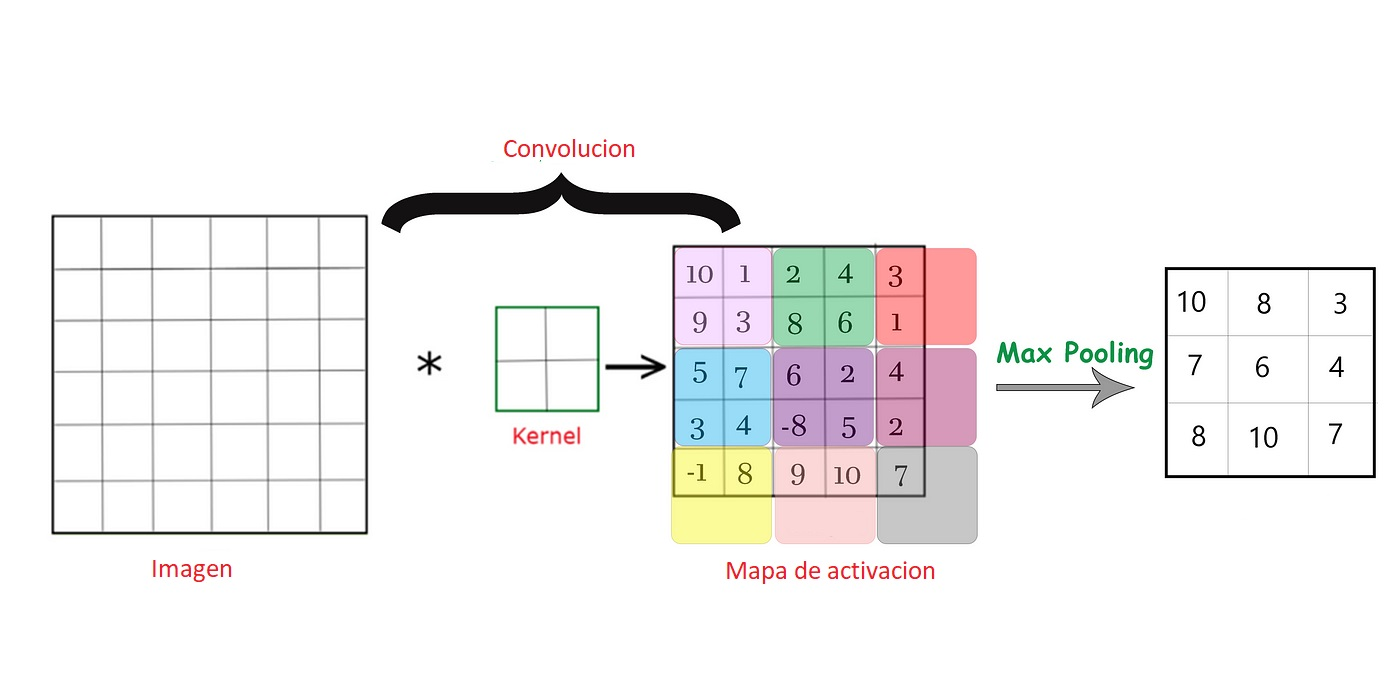
\includegraphics[width=1\textwidth]{imgs/ej-maxpooling.jpg}
    \caption{Ejemplo de funcionamiento de Maxpooling.}
    \label{fig:ejemplo-mp}
\end{figure}
 
Como capa siguiente se tiene un capa GlobalAvgPooling o Global Average Pooling, esta reemplaza las fully conect layers o capaz completamente 
conectada, por lo general se tiene una capa del tipo fully conect unida a todo los mapas de activacion, pero al colocar una capa GlobalAvgPooling
se busca obtener un unico mapa de activacion para cada categoria buscada,es decir se toma el promedio de cada mapa y se coloca en un vector directamente 
conectado a una funcion softmax. Esta configuracion reduce la necesidad de ajustar nuevos parametros por lo que se reduce la posibilidad de 
realizar overfitting(sobre entrenamiento) en la red.[https://arxiv.org/pdf/1312.4400.pdf]

Como capa final de la red se coloca una funcion Softmax, es una de las mas utilizadas como capa final de redes neuronales que buscan realizar
categorizacion, ya que esta permite obtener la probabilidad de obtener la categorizacion correcta dado que se sabe cual es la categoria correcta.
 
\section{Requerimientos necesarios de la red}
Una vez que tenemos las bases teoricas para comprender el funcionamiento de una CNN, vamos a meternos en los requerimientos propios que posee 
la red que es utilizada durante este trabajo, segun los datos provistos por el autor la red necesita como entrada una red imagen de la patente
en blanco y negro de dimensiones 70x140 pixeles.
Por lo que se ve que es necesario realizarle un tratamiento previo a las imagenes obtenidas antes de ingresalas por la red que realizara el 
algoritmo de OCR, el tratamiento necesario lo podemos ver en la \ref{fig:Comparativa-imagenes}.
\begin{figure}[!tbp]
 \centering
    \begin{subfigure}[b]{0.49\textwidth}
        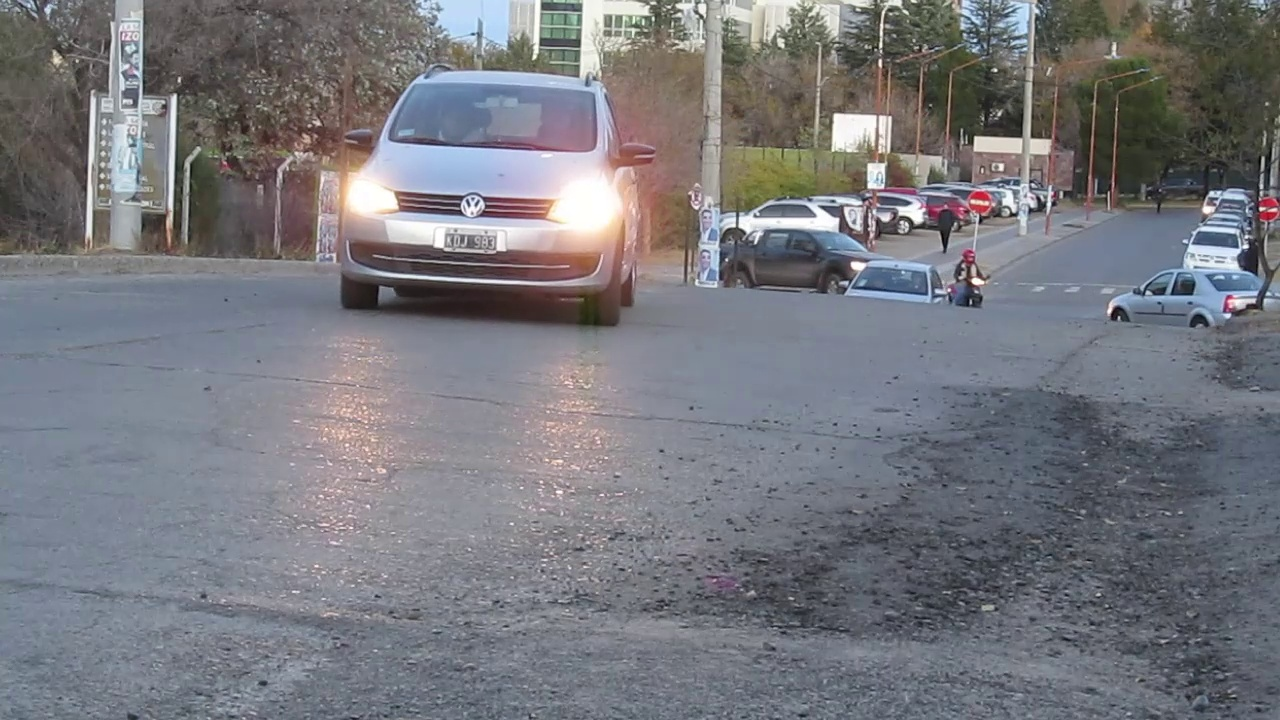
\includegraphics[width=\textwidth, height=\textwidth]{imgs/imagen-obtenida.jpg}
        \caption{Imagen obtenida por la camara.}
        \label{fig:imagen-obtenida}
    \end{subfigure}
    \hfill
    \begin{subfigure}[b]{0.49\textwidth}
        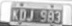
\includegraphics[width=0.7\textwidth, height=0.7\textwidth]{imgs/imagen-requerida.jpg}
        \caption{Imagen requerida por la red.}
        \label{fig:imagen-requerida}
    \end{subfigure}
 \caption{Compartiva imagenes a)Obtenida por la camara b)Requerida por la red.}
 \label{fig:Comparativa-imagenes}
\end{figure}

Para logralo, es necesario utilizar otra red nueronal, para que detecte la ubicacion de la patente, y asi poder realizar el recorte e ingresarla 
a la CNN para que obtenga los caracteres, dicha red es la Yolo (You Only Look Once ) en su version 4. 

Este difiere con otro tipo de detectores en que no utiliza la imagen completa y se queda con las regiones en la que obtuvo mayor puntaje y las 
considera como objeto detectado si no que, mediante una red neuronal tambien del tipo CNN toma la imagen completa, dibuja una serie de cuadrados
en diversas capas junto con su clasificacion, estas capas deben mesclarse para realizar la correcta deteccion, dicha implementacion se ve en la 
Fig. \ref{fig:funcionamiento-yolo}, una vez que se tiene la ubicacion del objeto una CNN clasifica la imagen. Esta implementación de YoloV4 
utiliza el marco Darknet.
\begin{figure}
    \centering
    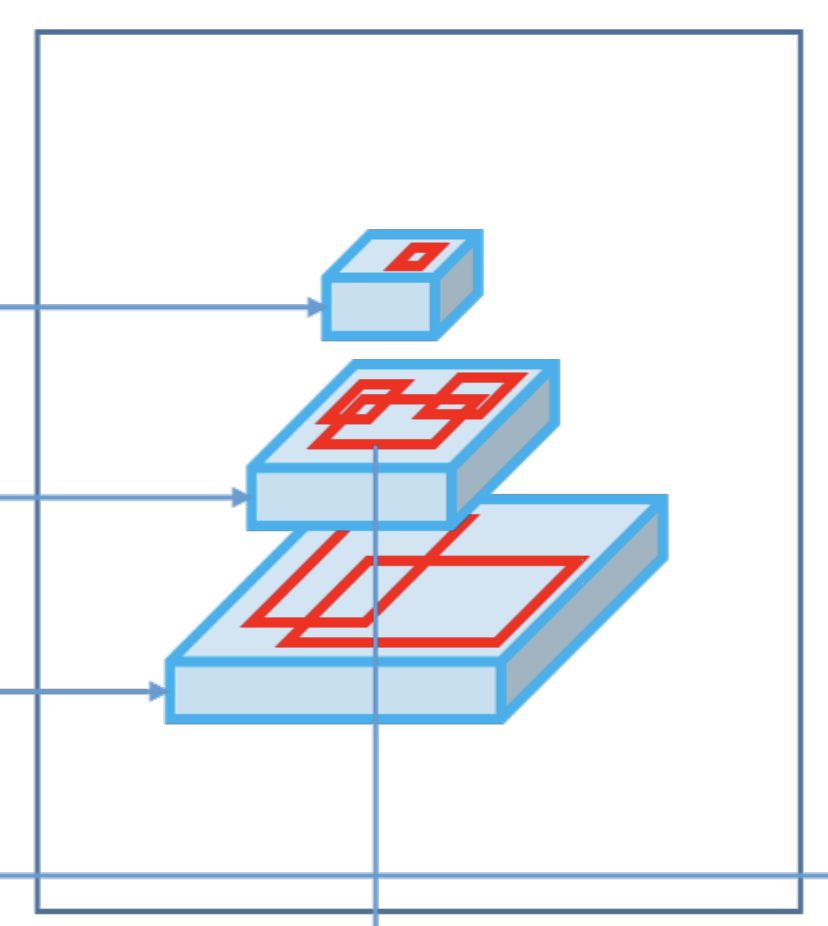
\includegraphics[width=0.5\textwidth]{imgs/funcionamiento-yolo.png}
    \caption{Funcionamiento del proceso de deteccion de la YoloV4.}
    \label{fig:funcionamiento-yolo}
    %%https://blog.roboflow.com/a-thorough-breakdown-of-yolov4/
\end{figure}

\section{Implementación del algoritmo en Python 3}

Para la implementacion del algoritmo se utilizo el lenguaje Python3, ya que este permite una rapida integracion de diversas librerias necesarias
para el funcionamiento del sistema completo, como es necesario el uso de una camara para la obtencion de las imagenes se utilizo la libreria 
OpenCv [https://github.com/opencv/opencv] para integrarla al algoritmo, a su vez como se requiere un activador para iniciar la camara, 
se construyo una libreria para usar un sensor de distancia ultrasonico US-100, esto se vera a detalle en la seccion siguiente.

Entonces la primer parte del algorimo se basa en la obtencion de la imagen, se espera la activacion del sensor mediante un umbral programable 
por el usuario y dependiendo de la ubicacion del conjunto sensor-camara, una vez que un vehiculo se detecta, se toma una imagen que dependiendo
del equipo que se este utilizando ya sea sensor SL o sensor SL mini, la existencia de estos 2 dispositivos se vera mejor en la siguiente 
seccion,se realizan 2 posibles acciones, en el caso del sensor SL, por su capacidades de hardware pueden correr dentro de el ambas redes, por lo
que el procesamiento de la imagen se realiza dentro de la propia placa, y se envia a un servidor sola la informacion relevante, como lo es la patente y 
la fecha y hora de ingreso o egreso dependiendo donde se encuentre el sensor. En el caso del sensor SL mini cuyas prestaciones de computo son 
inferiores este solo se encarga de tomar la foto y enviarla al servidor para que este procese la imagen y devuelva al sensor la habilitacion para el
ingreso o egreso.

En ambos casos la secuencia del algoritmo es la siguiente: 
\begin{itemize}
    \item cada un tiempo periodico se chequea si ingreso una nueva imagen para procesarla, esto se realiza mirando el contenido de una carpeta especifica.
    \item Cuando se encuentra una nueva imagen, se ingresa la imagen a la YoloV4, para que detecte la ubicacion de la patente, aqui ocurren 2 posibles acciones, si 
    se detecto patente se obtiene las coordenadas para realizar el recorte y en el caso de no detectar patente se envia un codigo de error al servidor y se descarta la imagen.
    \item se realiza el recorte de la imagen.
    \item Se envia la imagen de la patente recortada para la que la CNN realice la deteccion de caracteres.
    \item obtenida la patente se envia al servidor para los chequeos de validacion, y registro de horario.
    \item se recibe del servidor la validacion, y se admite la circulacion del vehiculo.
\end{itemize}




